\section{Related Work}
\label{related}

\subsection{Ibis}
\label{related-ibis}
\emph{Ibis} is an open source Java grid software project of the Computer Systems
group, which is part of the Computer Science department of the Faculty of
Sciences at the \emph{Vrije Universiteit}, Amsterdam, The Netherlands. The main
goal of the Ibis project is to create an efficient Java-based platform for grid
computing. The Ibis project currently consists of the IPL (a communication
library), a variety of programming models, the Java Grid Application Toolkit, and
the Zorilla peer-to-peer grid middleware. All components can be deployed on any
grid platform, due to the use of Java \cite{ibis-www}.

\subsubsection{JavaGAT}
\emph{Java Grid Application Toolkit} (JavaGAT) offers a set of coordinated,
generic and flexible APIs for accessing grid services from application codes,
portals, data managements systems, etc. \cite{javagat-www} JavaGAT sits between
grid applications and numerous types of grid middleware, providing uniform
interfaces for file operations, file stream operations, job submission,
monitoring, and access to information services (see Figure
\ref{related-gat-design}).

\begin{figure*}[ht] %[placement] where placement is h,t,b,p
\begin{center}
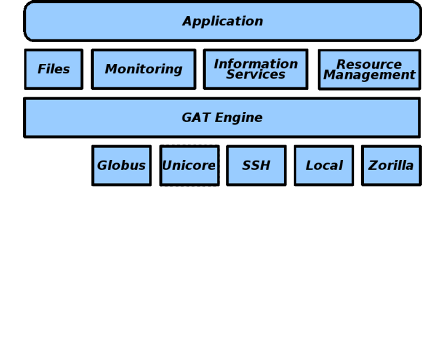
\includegraphics[width=10cm]{./figures/gat-design.png} 
\caption{The Structure of JavaGAT.\label{related-gat-design}}
\end{center}
\end{figure*}

As a result, grid application programmers need only to learn a single API to
obtain access to the entire grid. Due to its modular design, JavaGAT can easily
be extended with support for other grid middleware layers \cite{javagat-www}.

Grid applications do not use grid middleware directly. Instead, the
applications calls methods of the GAT API. The GAT engine dynamically `routes'
the API calls to the correct grid middleware. There are plugins (called
\emph{adaptors}) for many different grid middleware systems \cite{javagat-www}.

\subsubsection{IPL}
The \emph{Ibis Portability layer} (IPL) is a communication library specifically
designed for usage in a grid environment. It has a number of properties which
help to achieve its goal of providing programmers with an easy to use, reliable
grid communication infrastructure \cite{ibis-www}.

The Ibis Portability Layer (IPL) acts as a common interface for the different
programming models to the bottom implementation layer. Multiple implementations
are available. Some, such as \emph{TcpIbis using} 100\% Java code to ensure
portability, and some, such as the \emph{MPI} (Message Passing Interface) based
Ibis implementation taking advantage of local high speed networks using native
code \cite{ibis-www}.

As we will see in Section \ref{applications}, we will use our application
storage server for both Ibis projects mentioned above.

\subsection{The Google App Engine}
\label{related-appengine}
April 7, 2008 Google launched a free-of-charge cloud computing service called
the \emph{Google App Engine}. Google offers a platform for developing and
hosting web applications at Google's data centers. Google virtualizes
applications and distributes databases across multiple servers and data centers.

\subsubsection{The Runtime Environment}
As of April 8th 2009 \cite{app-engine-java} the Google App Engine provides two
programming languages to build and run web applications. Besides \emph{Python}
\cite{python-www}, also the \emph{Java} \cite{java-www} programming language is
featured to develop web applications and run them on Google's resources. Since
the feature of running your applications in Java is still relatively new, we
focused on the Python runtime environment for scientific purposes.

A Python web application interacts with the App Engine web server using the CGI
protocol. An application can use a WSGI-compatible web application framework
using a CGI adapter. App Engine includes a simple web application framework,
called \emph{webapp}, to make it easy to get started. For larger applications,
mature third-party frameworks, such as \emph{Django} \cite{django-www}, work
well with App Engine.

The App Engine currently only supports Python 2.5.2 (Python 3 is considered a
future release). The Python interpreter runs in a secured \emph{sandbox}
environment to isolate our application for service and security. The interpreter
can run any Python code, including Python modules we want to  include with our
application, as well as the Python standard library. The interpreter cannot load
Python modules with C code; it is a `pure' Python environment
\cite{app-engine-sandbox}.

In addition, Google also provides a distributed database, called the
\emph{datastore}. The datastore provides robust scalable data storage for our
application. The datastore is designed with web applications in mind, and
emphasizes on read and query performance. It stores data entities with
properties, organized by application-defined kinds. It can perform queries over entities of
the same kind, with filters and sort orders on property values and keys. All
queries are pre-indexed for fast results over very large data sets. The datastore
supports transactional updates, using entity groupings defined by the application
as the unit of transactionality in the distributed data network
\cite{app-engine-datastore}.

\subsubsection{Limitations}
Although the Google App Engine provides us with resources, it also has some
limitations we should consider. All applications hosted on the App Engine
servers, are run within a sandbox. Spawning new processes using \texttt{fork()}
or threads are not allowed. Application code only runs in response to a web
request, and must return response data within thirty seconds. After the response
is sent, no code execution can take place.

An application can only access other computers on the Internet through the
provided URL fetch and email services and APIs. No socket connections to other
machines can be made. Other computers can only connect to the application by
making HTTP (or HTTPS) requests on the standard ports.

An application cannot write to the file system. An app can read files, but only
files uploaded with the application code. The app must use the App Engine
datastore for all data that persists between requests.

\subsubsection{Quotas}
\label{appengine-quotas}
The Google App Engine is free of use up to a certain level of used resources,
after which fees are charged for additional storage, bandwidth or CPU cycles
required by the application. As of June 29th, 2009, quotas that are enforced by
Google are provided in Figure \ref{quota-table}. Note that the table below some
quotas are billable, if the user provides payment information using \emph{Google
Checkout} \cite{google-checkout-www}. When you enable billing for your app, the
app's fixed quotas increase and an optional maximum can be set by the
application's administrator (the latter are called \emph{billable quotas})
\cite{app-engine-quotas}.

\begin{figure}[h,t]
\begin{center}
\begin{tabular}{| l | l | l | }
\hline
\multirow{2}{*}{Resource (*=billable)} & \multicolumn{2}{|l|}{Free Default
Quota} \\
\cline{2-3}
& Daily Limit & Maximum Rate \\
\hline
Requests & 1,300,000 requests & 7,400 requests/minute \\
\hline
Outgoing Bandwidth* & 1 gigabyte & 56 megabytes/minute \\ 
\hline
Incoming Bandwidth* & 1 gigabyte & 56 megabytes/minute \\
\hline
CPU Time* & 6.5 CPU-hours & 15 CPU-minute/minute \\
\hline
Datastore API Calls & 10,000,000 calls & 57,000 calls/minute \\
\hline
Stored Data* & 1 gigabyte & None \\
\hline
\end{tabular}
\caption{Google App Engine Free Default Quotas. \label{quota-table}}
\end{center}
\end{figure}

Note that Google has the right and ability to change these quotas over time.
During the development of our project, this has happened several times, both
increasing and decreasing quotas.

\subsubsection{Monitoring}
For the administrativor to monitor the quota already used by other users, one can
login to the administration panel. All quotas as described above can be monitored
from this website, and additionally, one can see when quotas will be reset (being
midnight, Pacific time\footnote{Historical note: The 24-hour replenishment cycle
was introduced in December 2008. It replaced a more complicated system of
`continuous' replenishment, to make it easier to report and control resource
usage.}).  Besides the monitoring of quotas, also various logs are available
(e.g. error logs, debug logs, and access logs), and one can check the contents of
the datastore as well. For more information on the administration panel, we
suggest reading \cite{app-engine-admin}.

\subsection{Project Overview}
As far as we know, the Google App Engine has not been used as an application
storage server. Obviously, Google did not intend the App Engine to be used for
such purposes, hence the lack of spawning new processes or threads, or the
limited response time of a request. The most usable feature to us is the
distributed datastore, which could serve well as application storage
server (for Ibis). 

In addition to this server, we will write a Java client to communicate to the
server over HTTP(S), as can be seen from Figure \ref{related-overview}. Once
this library is imported into Ibis, Ibis applications can use the
library to store their data items in the data store. In the following sections
we will describe our project design in more detail.

\begin{figure*}[ht] %[placement] where placement is h,t,b,p
\begin{center}
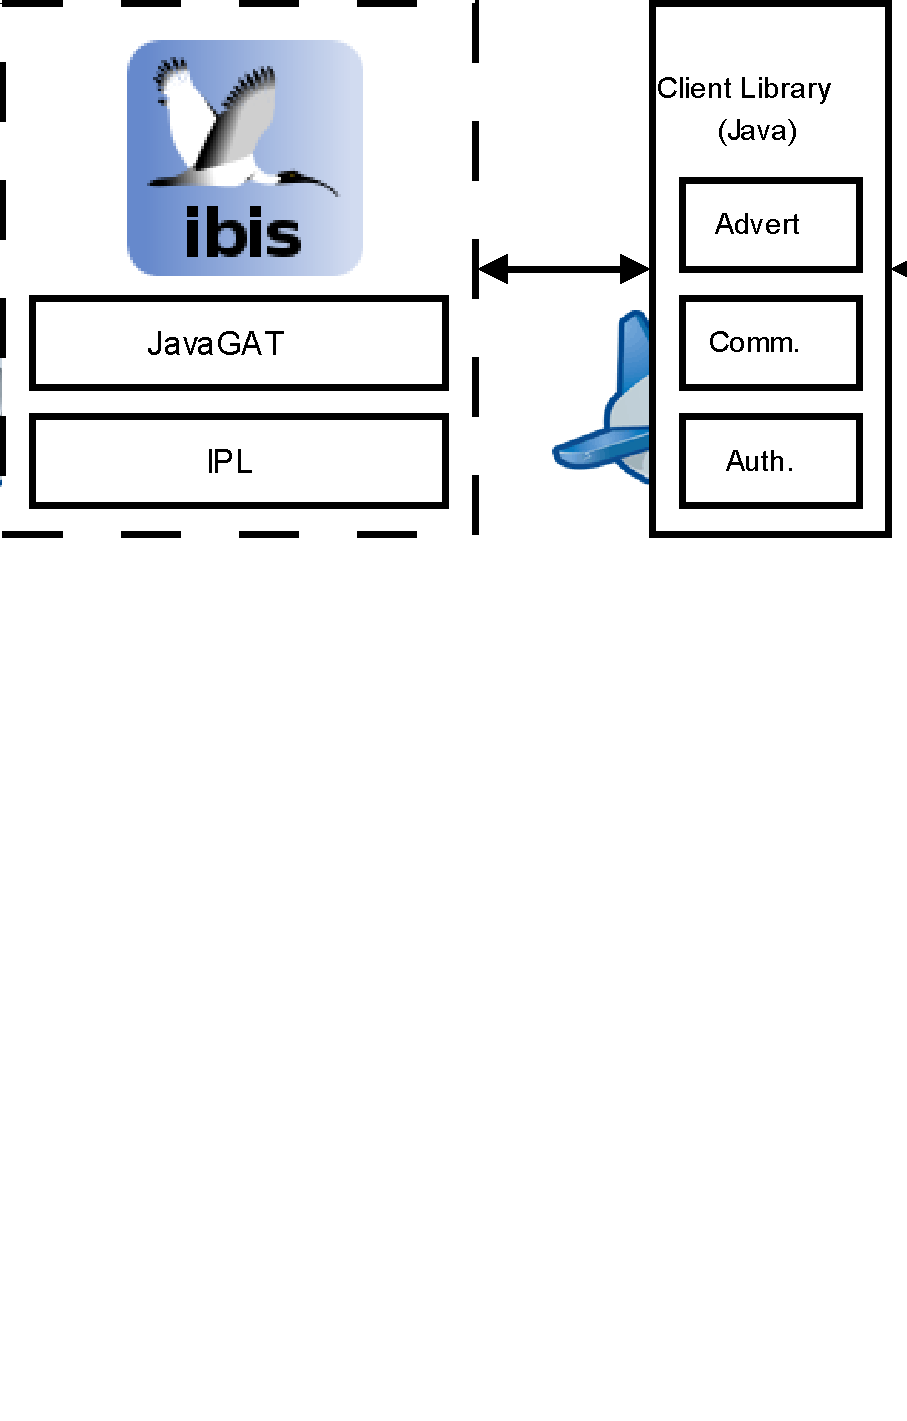
\includegraphics[width=14cm]{./figures/project_design.pdf} 
\caption{An Overview of our Project.\label{related-overview}}
\end{center}
\end{figure*}
